\subsection{Autoregressive Long Video Generation and Distillation}

\begin{figure}[H]
    \centering
    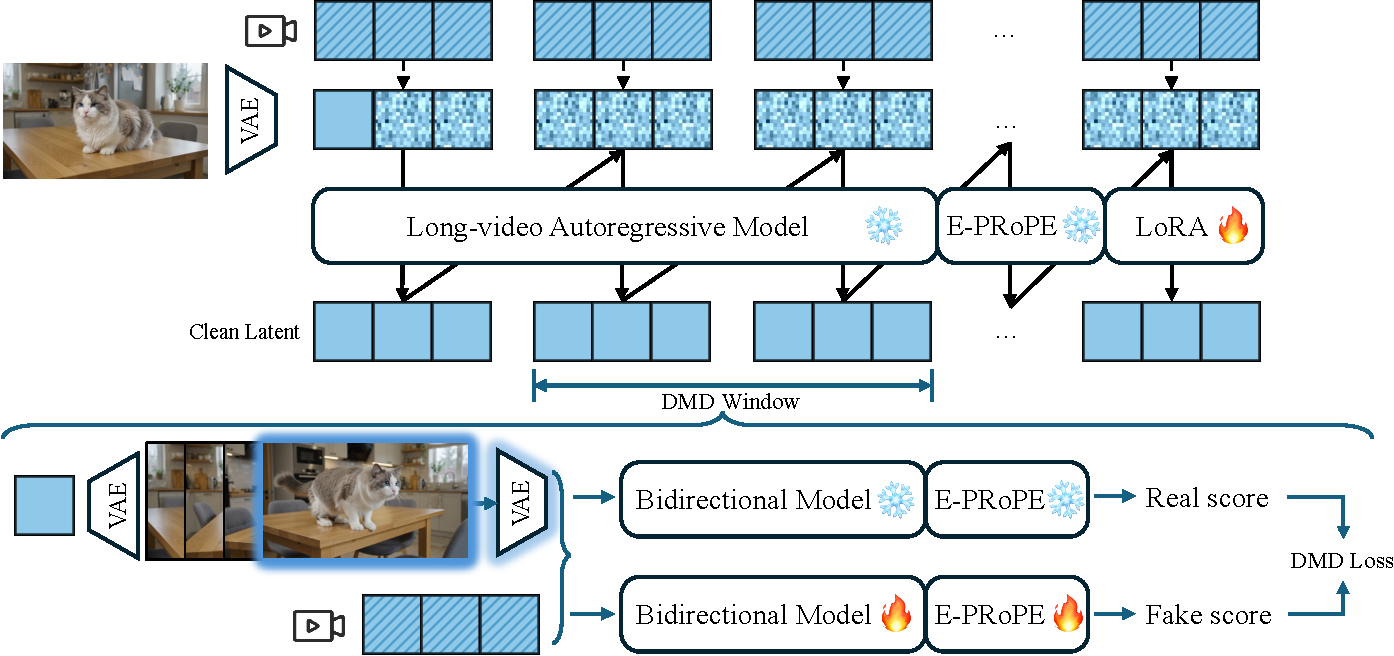
\includegraphics[width=0.8\linewidth]{figures/dmd_forcing_stage3-crop.pdf}
    \caption{DMD-forcing for camera-controlled long-video distillation. The E-PRoPE AR student is distilled from the bidirectional E-PRoPE teacher through DMD supervision over local temporal windows sampled from long videos, while preserving the streaming autoregressive sampling interface.}
    \label{fig:dmd-forcing}
\end{figure}

To enable few-step long-video generation, we distill a bidirectional model into an autoregressive generator that can stream from generated history while preserving visual quality and camera controllability.

We train few-step autoregressive model using causal forcing~\citep{huang2025selfforcing,zhu2026causalforcing} on large-scale high-quality video data, while keeping it close to the original visual distribution of the bidirectional model. 
Subsequently, following LongLive~\citep{yang2025longlive}, we further adapt the model on long sequences with long rollouts and local temporal windows, using Infinity-RoPE \citep{yesiltepe2025infinityrope} to support extended autoregressive context and reduce long-video failures such as identity drift, background mutation, and weakened prompt or motion control.

For camera-controlled generation, we incorporate an E-PRoPE branch into the long-video T2V student and distill the resulting few-step camera-controlled autoregressive model from a bidirectional E-PRoPE teacher. 
Although this branch enables camera control, chunk-wise inference may still lead to reduced motion smoothness and degraded camera controllability over long sequences. 

We therefore repeat the long-video DMD training to improve this behavior. 
Figure~\ref{fig:dmd-forcing} illustrates the DMD-forcing pipeline, in which camera-controlled student rollouts are matched to the bidirectional E-PRoPE teacher over local temporal windows sampled from long videos.

To preserve I2V quality, we perform I2V DMD distillation using the bidirectional E-PRoPE model as the teacher. The first latent frame of each sampled DMD window is decoded by the VAE and fed to the teacher as the image condition, enabling the teacher to supervise the camera-controlled AR student over local temporal windows of long videos.
With this design, the model can perform stable long-duration inference for videos up to one minute while maintaining camera controllability and temporal coherence across chunks.
